
\chapter{Mining}

Meedoen aan de proof-of-work loterij om de mogelijkheid tot het aanpassen van het bitcoin-grootboek te winnen, is beter bekend als \textit{minen}. Dit is hoe het werkt:

\begin{enumerate}
    \item Iedereen die wil deelnemen, sluit zich aan bij het bitcoinnetwerk door hun computer aan te zetten, de juiste bitcoin-software te draaien en te luisteren naar anderen die hun transacties aankondigen.
    \item Alice kondigt haar voornemen aan om wat munten naar Bob te sturen. De computers op het netwerk \textquotedbl{}roddelen\textquotedbl{} met elkaar om deze transactie naar iedereen op het netwerk te verspreiden.
    \item Alle computers die willen deelnemen aan de loterij starten met het \textit{hashen} van de transacties waar ze over hebben gehoord door willekeurige \textit{nonces} toe te voegen aan de transactielijst en de sha256 \textit{hash}-functie uit te voeren.
    \item Gemiddeld elke tien minuten vindt een computer een hash afgeleid van de transacties die lager is dan het huidige doelnummer en wint daarmee de loterij.
    \item Deze computer maakt zijn winnende getal bekend, evenals de invoer (transacties en nonce) die ze hebben gebruikt om het winnende lot te produceren. Het kan uren gekost hebben om dat te vinden, of een paar minuten. Deze informatie bij elkaar (transacties, nonce en de hash van het proof-of-work) wordt een \textit{blok} genoemd.
    \item Alle andere deelnemers valideren het blok door te controleren of de transacties in het blok samen met de nonce inderdaad hashen tot wat er gedeeld wordt, dat de hash inderdaad lager is dan het doelnummer, dat het blok geen ongeldige transacties bevat én dat de geschiedenis in het blok niet in strijd is met voorgaande blokken.
    \item Iedereen schrijft het blok in zijn kopie van het grootboek en voegt het toe aan de bestaande ketting van blokken, bekend als een \textit{blockchain}.
\end{enumerate}

Dat is het in een notendop. We hebben ons eerste blok geproduceerd en mogen onze eerste transacties aan onze grootboeken toevoegen.

Misschien heb je in de media de vaak herhaalde bewering gelezen dat bitcoin mining het oplossen van ingewikkelde vergelijkingen inhoudt. Nu zul je begrijpen dat dit volstrekt onjuist is; in plaats van vergelijkingen op te lossen, moet je bij bitcoin mining herhaaldelijk gooien met een grote virtuele dobbelsteen om een hash te produceren die onder een bepaald doelnummer valt. Het is gewoon een kansspel dat deelnemers dwingt om een bepaalde hoeveelheid elektriciteit te verbruiken.

\section{Hoe worden nieuwe bitcoins gemaakt?}

Tot nu toe hebben we besproken hoe Alice \$2 naar Bob kan sturen. We gaan vanaf nu stoppen met praten over dollars, want bitcoin kent geen dollars. Wat we wel hebben, zijn bitcoins zelf: digitale eenheden die waarde vertegenwoordigen op het bitcoinnetwerk.

Om bij ons voorbeeld te blijven, kunnen we zeggen dat Alice 2 bitcoins naar Bob stuurt door aan te kondigen dat ze haar munten, die op haar \textquotedbl{}rekening\textquotedbl{} staan, naar die van Bob overzet. Vervolgens wint iemand de proof-of-work loterij, en wordt haar aangekondigde transactie toegevoegd aan het grootboek.

Maar waar kwamen die 2 bitcoins van Alice oorspronkelijk vandaan? Hoe ging bitcoin van start en hoe verwierf iemand ooit munten voordat er marktplaatsen waren om ze te kopen met traditionele fiatvaluta zoals dollars of euro’s?

Toen Satoshi bitcoin ontwierp, had hij ervoor kunnen kiezen om een database te maken die alle 21 miljoen munten aan hem toewees en vervolgens iedereen te vragen ze van hem te kopen. Echter zou er weinig reden zijn voor anderen om waarde toe te kennen aan een systeem waarin één enkeling alle waarde bezat. Hij kon een register gemaakt hebben waar mensen konden intekenen met een e-mailadres om kans te maken op enkele munten. Maar een registratiesysteem zou vatbaar zijn aan een zogenaamde \textit{Sybil-aanval}, aangezien het quasi gratis is om miljoenen e-mailadressen aan te maken.\footnote{Een Sybil-aanval is een aanval waarin een deelnemer aan een bepaald netwerk een groot aantal pseudonieme addressen aanmaakt om een grote hoeveelheid invloed in het netwerk te vergaren; vernoemd naar Sybil, een boek over een vrouw met een dissociatieve identiteitsstoornis}

Satoshi koos uiteindelijk om de nieuwe munten te laten genereren door het proces van minen, oftewel de deelname aan de proof-of-work loterij om het recht te verkrijgen in het grootboek te schrijven. Wanneer je een grote hoeveelheid energie gebruikt en het winnende getal van het volgende geldige blok vindt, krijg je het recht om de transacties die bij jou bekend zijn toe te voegen aan het grootboek. Daarbovenop mag je ook een speciale transactie toevoegen aan het blok die we een \textit{coinbase}-transactie noemen. Zo’n transactie zegt: \textquotedbl{}12,5 bitcoin werden gemaakt en toegekend aan Marie de Miner om haar te compenseren voor de energie die gebruikt werd om het blok te vinden.\textquotedbl{}

Dit is hoe nieuwe bitcoins \textquotedbl{}gemaakt\textquotedbl{} worden. Met dit proces is iedereen ter wereld in staat om hun eigen munten te vergaren zonder tussenkomst van een centrale autoriteit én zonder hun identiteit bekend te moeten maken. De enige vereiste is dat ze genoeg willen betalen voor de elektriciteit die nodig is om mee te doen met de loterij. Dit maakt bitcoin’s uitgifte resistent tegen \textit{sybil}-aanvallen. Wie munten wil, zal energie moeten verbruiken en iets moeten betalen om ze te maken.

\section{De blokbeloning}
De persoon die de loterij wint, mag zichzelf enkele vers gemaakte munten toekennen. Maar waarom is de beloning 12,5 bitcoins en niet 1000? Waarom kan niemand valsspelen en zichzelf een willekeurig bedrag toekennen?

Bitcoin is een systeem van gedistribueerde consensus. Dit betekent dat iedereen akkoord moet gaan met wat geldig is en wat niet. Dat kan door software op je computer te draaien die een bekende set van regels afdwingt. Deze regels staan bekend als de consensusregels van bitcoin. Wanneer een miner een nieuw blok vindt, wordt alles tegen de consensusregels afgewogen. Wanneer het blok geldig blijkt te zijn, schrijft iedereen het in hun grootboek en wordt het geaccepteerd als waarheid. Indien niet, dan wordt het blok verworpen.

Hoewel de volledige lijst van consensusregels vrij complex is, kunnen we de belangrijkste hieronder opsommen:

\begin{itemize}
    \item Een geldig blok mag een specifieke hoeveelheid nieuwe munten aan het netwerk toevoegen, zolang het voldoet aan de regels van het uitgifteschema wat vastgelegd is in de software.
    \item Transacties moeten geldige handtekeningen hebben die aangeven dat de eigenaar het verzenden daadwerkelijk goedgekeurd heeft.
    \item Transacties die munten proberen uitgeven die al eerder uitgegeven werden, kunnen onder geen geval plaatsvinden.
    \item De hoeveelheid data in het blok mag een specifieke limiet niet overschrijden.
    \item De proof-of-work hash van het blok moet kleiner zijn dan het huidige doelnummer, waardoor onbetwistbaar aangetoond wordt dat dit blok tot stand kwam door een bepaalde hoeveelheid elektriciteit te gebruiken.
\end{itemize}

Indien Marie een blok vindt en beslist om zichzelf een beetje extra te geven, dan zullen de computers van de overige deelnemers dit blok afwijzen en als ongeldig beschouwen. Dit komt omdat de bitcoin-software die iedereen draait een stukje code bevat dat zegt: “de huidige blokbeloning is precies 12,5 bitcoins. Als je een blok ziet waarin iemand meer dat dit bedrag toekent, verwerp het dan.”

Als Marie probeert vals te spelen en een ongeldig blok produceert, dan komt het blok in niemands grootboek terecht en zal ze simpelweg veel elektriciteit verspild hebben om een vervalsing te produceren die niemand wil. Dit geeft bitcoin een \textit{onvervalsbare kostbaarheid}, een term die werd geïntroduceerd door Nick Szabo in zijn esssay \textquotedbl{}Shelling Out\textquotedbl{}. Het is vrij makkelijk te begrijpen dat geld wat makkelijk te vervalsen is, nooit daadwerkelijk nuttig kan zijn als geld. Het is onmogelijk om bitcoin te vervalsen omdat iedere munt op echtheid te controleren valt met een simpele, wiskundige test.

Satoshi ontgon het eerste \textquotedbl{}genesis\textquotedbl{} blok, wat de eerste bitcoins ooit produceerde. De code is \textit{open source} en dus kan iedereen een kijkje onder de motorkap nemen om te zien of er niets verkeerd loopt. Maar zelfs Satoshi moest miljarden berekeningen doen en meespelen met de proof-of-work loterij om die eerste blokken te vinden. Op geen enkele manier kon hij een vervalsing produceren door te liegen over de energie die hij nodig had om een winnende oplossing te vinden. En dat terwijl hij de ontwerper van het systeem was.

Iedereen die zich daarna bij het netwerk aansloot kon controleren dat zijn gevonden oplossingen voldeden aan de vereisten. Door ze naast het initiële doelnummer en transactiedata te leggen, blijkt overduidelijk dat een bepaalde hoeveelheid energie gebruikt werd om een statistisch zeldzaam doelnummer te vinden. Stel je voor dat het mogelijk is om met diezelfde precisie en regelmaat te controleren hoe fiatvaluta in het traditionele bankensysteem tot stand komt.

\section{De halvering}
Het proces van minen produceert nieuwe bitcoins. Maar Satoshi wou een systeem waarin het onmogelijk was om de waarde van de munt te devalueren. Hij wou niet dat het monetaire aanbod tot in het oneindige zou blijven stijgen. In plaats daarvan, ontwierp hij een uitgifteschema dat snel begon en geleidelijk afneemt tot uiteindelijk geen nieuwe munten meer zullen worden geproduceerd.

In het begin was de beloning voor een blok 50 bitcoin en dat is hoeveel Satoshi ontving voor zijn allereerste ontgonnen blok. Net zozeer kregen alle andere deelnemers die zich aansloten bij het netwerk in de begindagen voor elke gevonden blok 50 bitcoin.

De bitcoin-software dwingt iedere vier jaar een halvering van de blokbeloning af. De periode is gebaseerd op het aantal blokken in plaats van een bepaalde periode van tijd, maar omdat blokken ongeveer elke tien minuten worden geproduceerd, maakt dit in werkelijkheid weinig verschil. In 2008 was de blokbeloning 50 BTC, in 2012 was het 25 BTC, in 2016 12,5. Vandaag, op 8 juni 2019, zijn al 579.856 blokken ontgonnen sinds het begin van bitcoin en is de beloning 12,5 BTC per blok.

Binnen 50.144 blokken, ongeveer in mei 2020, zal de beloning verlaagd worden tot 6,25 BTC per blok. De jaarlijkse toename van het aanbod wordt dan ongeveer 1,8\%. Na nog eens 12 jaar, 3 halveringen later, zullen 99\% van alle bitcoins in circulatie zijn en krijgen miners nog minder dan 1 bitcoin per gevonden blok. Je kan de voortgang van de halveringen volgen op \href{https://bitcoinblockhalf.com}{https://bitcoinblockhalf.com}.

\begin{figure}
    \centering
    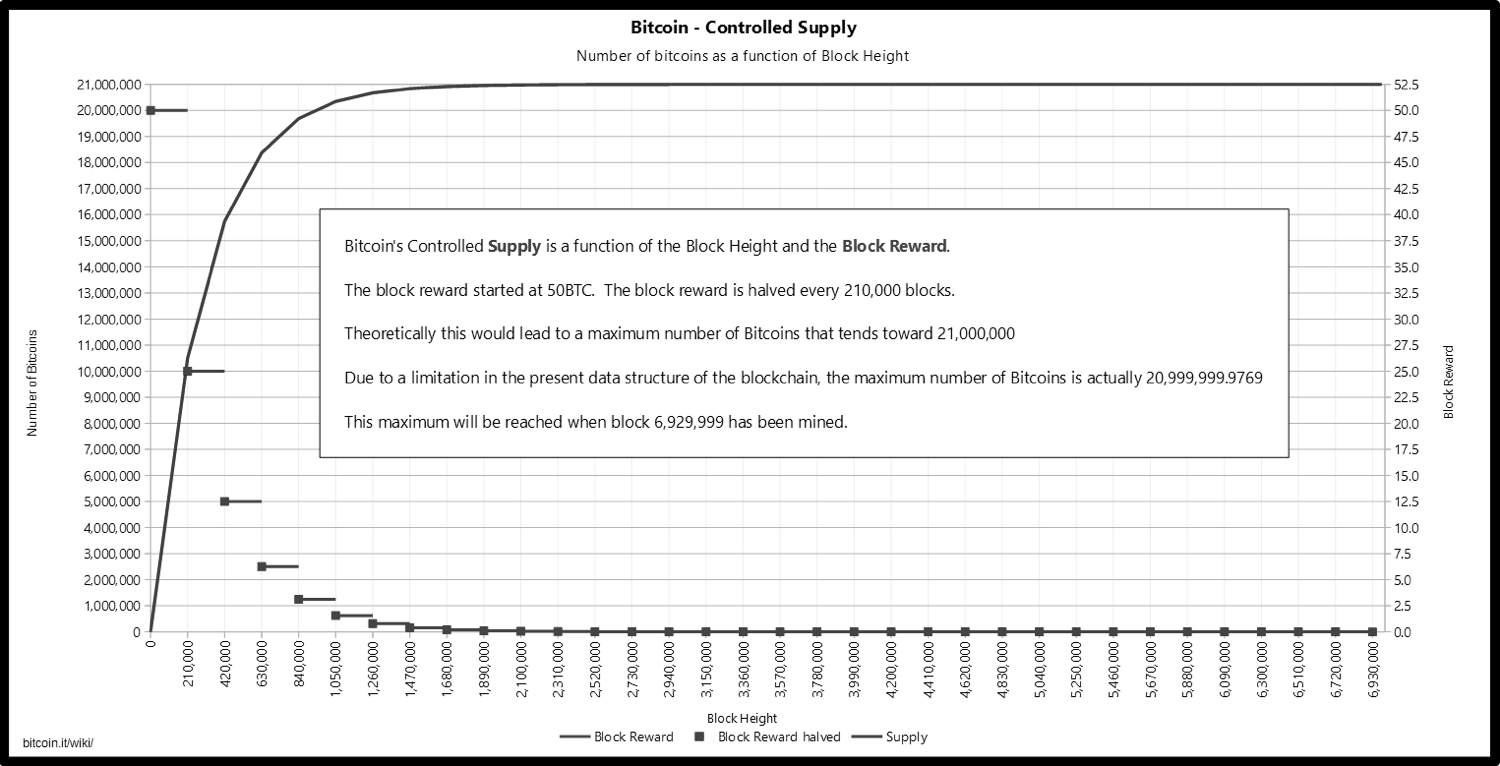
\includegraphics[width=\textwidth]{images/fig6.png}
    \caption{\footnotesize{\textit{Het gecontroleerde monetaire tijdschema van bitcoin kan door iedereen worden bevestigd.}}}
    \label{fig6}
\end{figure}

Uiteindelijk, rond het jaar 2140, zal de blokbeloning volledig wegvallen en moeten miners genoegen nemen met transactievergoedingen van de gebruikers als compensatie voor hun werk.

De blokbeloningen, en het uitgifteschema in het algemeen, worden afgedwongen in de bitcoin-software die, zoals eerder gesteld, volledig \textit{open source} is en dus door iedereen volledig gevalideerd kan worden. Een blok produceren dat niet voldoet aan de regels zal door niemand met dezelfde software geaccepteerd worden.

\section{Beheersen van de uitgifte en het blokinterval}

Het minen van bitcoin vereist computers en elektriciteit. Dus hoe meer computers en elektriciteit je ter beschikking hebt, hoe groter de kans is dat jij een winnend lot weet te vinden. Stel, het netwerk bestaat uit 100 computers met gelijke rekenkracht en jij bezit daar 10 van. Dit betekent dat je in ongeveer 10\% van de gevallen een winnende oplossing zal vinden. Maar mining is een proces waar geluk en willekeur mee gemoeid gaat. Het is dus theoretisch gezien mogelijk dat er uren of dagen voorbijgaan zonder dat je een winnend lot vind.

In het vorige deel hebben we uitgelegd dat miners zichzelf niet simpelweg een arbitraire blokbeloning kunnen toekennen. Die zouden door andere \textit{nodes} verworpen worden. Maar wat als ze een heleboel energie gebruikten om het miningproces sneller te laten verlopen en zo meer bitcoins te verwerven? Dit zou in strijd zijn met het opzet in het ontwerp van bitcoin, namelijk dat het uitgifteschema van tevoren bekend zou moeten zijn.

Laten we opnieuw het eerder gegeven voorbeeld nemen: er zijn 1000 mogelijke hashes en ons doelnummer is 100. In 10\% van de gevallen zullen we een getal vinden dat kleiner is dan 100 en een geldig blok vinden.

Stel dat het 1 seconde duurt om elke hash te berekenen. Als we iedere seconde “onze dobbelsteen rollen” door de huidige transacties en onze lukrake \textit{nonce} te hashen, vinden we in 10\% van de keren een getal dat kleiner is dan het doelnummer. We verwachten dus dat het ons gemiddeld 10 seconden vergt om een geldige hash te vinden.

Wat gebeurt er wanneer 2 computers meedoen aan de loterij? Ze hashen dan dubbel zo snel en verwachten een geldige hash iedere 5 seconden. Wat als 10 computers meedoen? Elk van hen kan ongeveer iedere seconde een winnende oplossing vinden.

Het probleem is dus het volgende: als meer mensen meedoen, worden blokken te snel geproduceerd. Dit leidt tot twee uitkomsten die we niet willen:

\begin{enumerate}
    \item Het is niet meer mogelijk om een vooraf vastgesteld uitgiftescheme aan te houden. We willen hiervoor ieder uur een relatief consistent aantal bitcoins in circulatie zien komen om te zorgen dat het proces tot in het jaar 2140 duurt, en niet eerder ten einde komt.
    \item Het creëert problemen op het netwerk: wanneer blokken te snel gevonden worden en geen tijd hebben om de rest van het netwerk te bereiken voordat een volgend blok gevonden wordt, kunnen we niet tot consensus komen over de lineaire geschiedenis van transacties. Verschillende miners zouden dan transacties in hun blokken gestopt kunnen hebben, die al uitgegeven werden in een vorig blok waar ze nog niet van op de hoogte waren.
\end{enumerate}

Als minder mensen minen dan hebben we het tegenovergestelde:

\begin{enumerate}
    \item Nieuwe bitcoins worden te traag uitgegeven waardoor het uitgifteschema niet klopt.
    \item Het systeem wordt onbruikbaar omdat je soms uren, dagen of langer zal moeten wachten om je transacties in het grootboek te krijgen.
\end{enumerate}

Het totale aantal hashes per seconde van alle miners op het netwerk noemen we de \textit{hash-rate}.



\begin{figure}
    \centering
    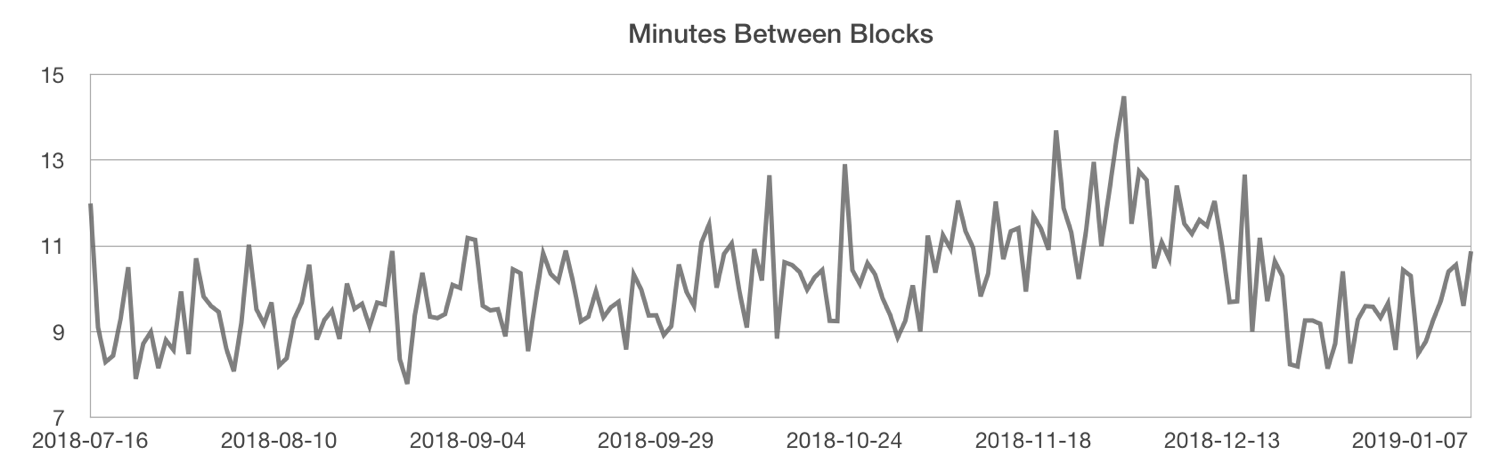
\includegraphics[width=\textwidth]{images/fig7.png}
    \caption{\footnotesize{\textit{De tijd tussen blokken varieert afhankelijk van de hash-rate die komt en gaat, evenals willekeurige kans.}}}
    \label{fig7}
\end{figure}


\section{Moeilijkheidsaanpassing: consensus over het doelnummer}

Aangezien bitcoin een vrijwillig en permissieloos systeem is waar mensen deel aan kunnen nemen zoals zij willen, zonder dat iemand de leiding heeft, zal het aantal miners op het netwerk sterk schommelen. We hebben een manier nodig om de productie van blokken stabiel te houden in plaats van telkens een versnelling of vertraging in productie te zien wanneer miners zich aansluiten of verdwijnen.

Hoe kunnen we het moeilijker maken om geldige hashes te vinden als meer spelers meedoen aan de loterij en makkelijker wanneer spelers weggaan? Op die manier zouden we de uitgifte en blokintervallen stabiel kunnen houden.

Herinner je dat het minen van bitcoin een loterij is waarin je een willekeurig getal moet vinden dat kleiner is dan het doelnummer.


\begin{figure}
    \centering
    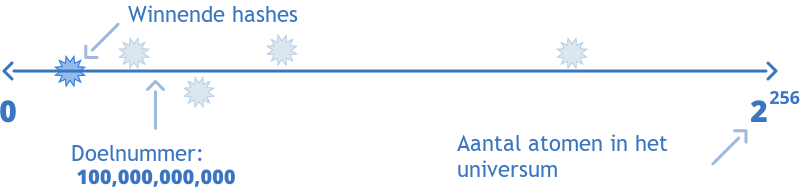
\includegraphics[width=\textwidth]{images/fig5.png}
    \caption{\footnotesize{\textit{We proberen deze kleine ruimte te raken. Het aantal mogelijke uitkomsten is extreem groot, dus het zal heel lang duren om daar te komen door willekeurige worpen van de dobbelsteen.}}}
    \label{fig8}
\end{figure}


Bitcoin lost dit probleem op door middel van een \textit{aanpassing van de moeilijkheidgraads}. Omdat iedereen dezelfde code draait die dezelfde regels afdwingt, én iedereen een volledige kopie heeft van de transactiegeschiedenis, kan iedereen onafhankelijk berekenen hoe snel blokken op dat moment geproduceerd worden.

Telkens wanneer we 2016 blokken geproduceerd hebben (ongeveer 2 weken)\footnote{De aanpassingsperiode van 2016 blokken is op basis van het beoogde blokinterval van 10 minuten; 10 minuten x 2016 blokken = twee weken. Het blokinterval werd arbitrair vastgesteld door Satoshi om groot genoeg te zijn zodat de meeste nodes kunnen op de hoogte zijn van de laatste blok. De periode van twee weken is ook ietwat arbitrair gekozen, maar is ontworpen om te voorkomen dat het spel belazerd wordt door te snelle achtereenvolgende aanpassingen in de hash-rate.}, analyseren we de snelheid van uitgifte over de afgelopen periode. We kijken hoeveel tijd nodig was om die 2016 blokken te produceren en passen vervolgens passen het doelnummer aan om de productie van blokken te versnellen of te vertragen.

Iedereen neemt de laatste 2016 blokken en deelt ze door de tijd die gemiddeld nodig was om te ze creëren. Was het gemiddelde meer dan 10 minuten? Dan gaan we te traag. Lag het gemiddelde onder de 10 minuten? Dan gaan we te snel.

We kunnen nu het doelnummer aanpassen zodat het groter of kleiner is, proportioneel met hoe traag of snel we gaan, om te zorgen dat we in lijn blijven met het afgesproken interval van 10 minuten.

Het doelnummer kan een groter getal worden, waardoor een groter bereik van hashes een geldige oplossing wordt. Hierdoor wordt de kans om een winnende hash te vinden voor de miners groter en hoeven ze minder energie te gebruiken om een blok te vinden. Dit heet \textit{de moeilijkheidsgraad verlagen}.

\begin{figure}
    \centering
    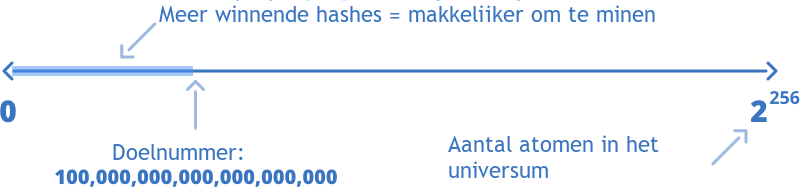
\includegraphics[width=\textwidth]{images/fig8.png}
    \caption{\footnotesize{\textit{Het verhogen van het doel vergroot de geldige ruimte, waardoor het waarschijnlijker wordt om in minder pogingen een juiste oplossing te vinden. Daardoor wordt het goedkoper in verbrande \mbox{energie.}}}}
    \label{fig9}
\end{figure}



Anderzijds, kunnen we het doelnummer kleiner maken zodat er minder hashes geldig zijn en miners meer energie moeten spenderen om een blok te vinden. Dit heet \textit{de moeilijkheidsgraad verhogen}.

Dit betekent dat we voor elke periode van 2016 blokken precies weten wat het doelnummer is. Het geeft ons de magische grens waarbinnen een hash van de proof-of-work moet vallen om een winnend lot te bemachtigen, binnen die periode.

De aanpassingen van de moeilijkheidsgraad en het doelnummer is misschien wel de belangrijkste innovatie van bitcoin. Het stelt iedereen in staat om onafhankelijk de lotnummers te verifiëren, die op hun beurt weer gebaseerd zijn op een doelnummer dat ook onafhankelijk te verifiëren is. Hierdoor kunnen we een loterij spelen zonder dat iemand ons de winnende combinatie hoeft te vertellen.



In Figuur \ref{fig10} zie je de \textit{hash-rate} (lijn) en de moeilijkheidsgraad (staven) doorheen de tijd. De moeilijkheid wordt iedere 2016 blokken aangepast en lijkt een beetje op een trap. Telkens wanneer de hash-rate boven de moeilijkheid uitstijgt, zie je dat de moeilijkheidsgraad stijgt om bij te benen. Wanneer de hash-rate zakt, zoals tussen oktober en december 2018, zakt ook de moeilijkheidsgraad. De aanpassing van de moeilijkheidsgraad volgt altijd wat de hash-rate doet met een vertraging van 2016 blokken (twee weken).

\begin{figure}
    \centering
    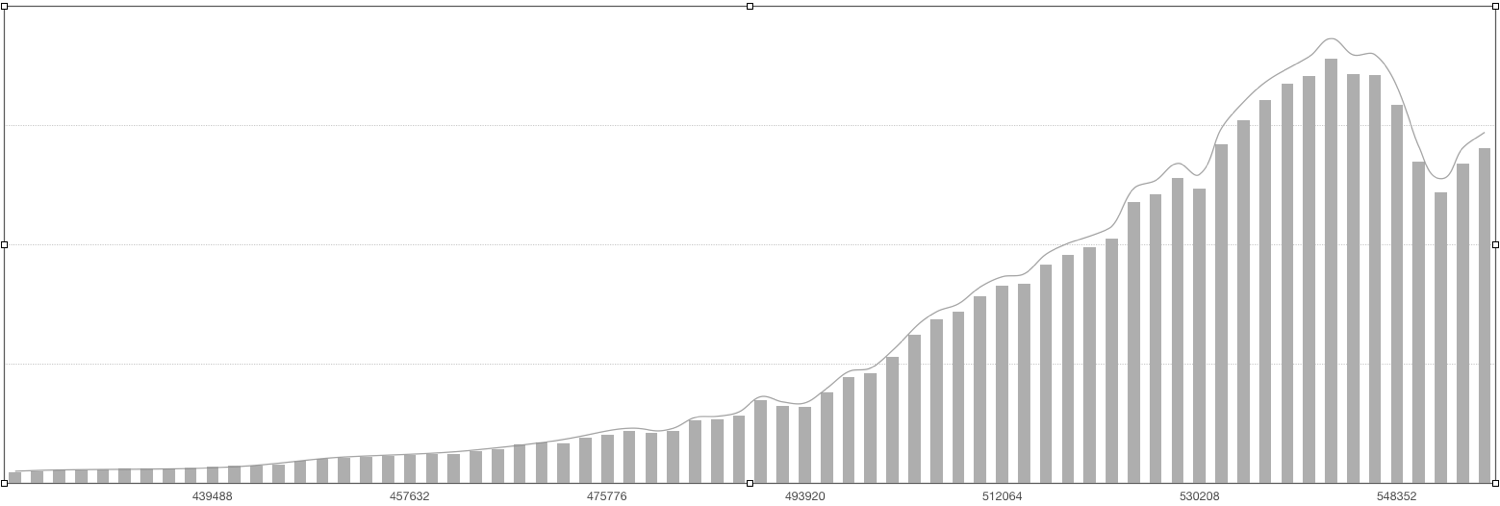
\includegraphics[width=\textwidth]{images/fig10.png}
    \caption{\footnotesize{\textit{Hash-snelheid versus moeilijkheid.}}}
    \label{fig10}
\end{figure}

Omdat er een vertraging van 2016 blokken op de aanpassing zit, is het mogelijk dat grote pieken omhoog of omlaag in hash-rate leiden tot een over- of onderproductie van bitcoins tijdens dat interval en licht afgeweken wordt van het uitgifteschema.

Het verhogen van de hash-rate gaat gepaard met de productie van een grote hoeveelheid nieuwe hardware, waardoor pieken relatief ongebruikelijk zijn en niet al te veel impact hebben. Het effect van iedere piek, omhoog of omlaag, zal beperkt blijven tot dat interval van 2016 blokken. Na de volgende aanpassing komen we opnieuw bij een gemiddelde van 10 minuten per blok.

\section{Hash-rate en de dollarwaarde van bitcoin}
Bitcoin herberekent de moeilijkheidsgraad automatisch op basis van alle rekenkracht van de loterijspelers. Dit zijn de miners die energie verbruiken om te hashen. Op die manier raakt de echte wereld vervlochten met onze digitale wereld. De prijs van bitcoin, de prijs van hardware en energie en de moeilijkheid van het doelnummer creëren feedback-koppelingen:

\begin{enumerate}
\item Speculanten kopen bitcoin omdat ze denken dat de prijs hoger gaat, waardoor ze de prijs opdrijven tot \$X.
\item Miners verbruiken tot \$X aan energie en hardware om bitcoins te verdienen.
\item Een grote vraag van kopers duwt de prijs omhoog en leidt tot meer miners die aardig verdienen aan hun activiteit.
\item Meer miners betekent meer hash-rate en meer verbruikte energie om bitcoin te produceren. Het netwerk wordt nog sterker beveiligd. De kopers worden gerustgesteld door de veiligheid van het netwerk en drijven de prijs soms nog verder omhoog.
\item Na 2016 blokken gaat de moeilijkheidsgraad omhoog door de aanwezigheid van meer hash-rate.
\item Een hogere moeilijkheid betekent een lager doelnummer. De miners vinden nu minder vaak blokken waardoor sommigen meer dan \$X spenderen in kosten om een bitcoin te minen.
\item Voor sommige miners blijkt het niet meer interessant om te minen, omdat ze meer energie verbruiken dan de winst die hun activiteit oplevert wanneer ze hun bitcoin verkopen. Ze leggen hun machines af en de hash-rate op het netwerk gaat terug omlaag.
\item De volgende 2016 blokken passeren. De moeilijkheid wordt opnieuw berekend en aangezien sommige miners offline gingen, wordt het deze keer makkelijker. Het doelnummer gaat omhoog.
\item De lagere moeilijkheid betekent dat miners, die voorheen onrendabel waren, hun machines terug aanzetten of dat nieuwe miners op het toneel verschijnen.
\item Ga terug naar 1.
\end{enumerate}
In een neerwaartse markt kan de cyclus in de andere richting gaan. Gebruikers van het netwerk dumpen dan hun munten, de prijs gaat omlaag en miners worden onrendabel.

Het algoritme voor de aanpassing van de moeilijkheidsgraad zorgt dat er altijd een evenwicht wordt gevonden tussen de prijs en de hoeveelheid hash-rate die aanwezig is op het netwerk. Zelfs als de prijs drastisch zou zakken en de helft van de huidige hash-rate uit het netwerk zou duwen, dan zou de volgende aanpassing het opnieuw rendabel maken op een nieuw evenwichtsniveau.

De aard van de moeilijkheidsaanpassing duwt inefficiënte miners eruit ten voordele van degenen die werken met de goedkoopst mogelijke energie en met de laagste totale operationele kosten. Na verloop van tijd dwingt het bitcoin miners richting afgelegen hoeken op de planeet. Ze gebruiken energiebronnen die onderbenut of volledig onontgonnen zijn. Een rapport van CoinShares uit 2019 schat dat ongeveer 75\% van de bitcoin miners hernieuwbare energie gebruikt.\footnote{Lees meer over de laatste stand van zaken betreffende mining op \href{https://coinshares.com/research/bitcoin-mining-network-june-2019 }{https://coinshares.com/research/bitcoin-mining-network-june-2019 }}

De laatste jaren ging de prijs pijlsnel omhoog, net als de totale hash-rate. Hoe hoger de hash-rate, hoe moeilijker het is om het netwerk aan te vallen. Om te bepalen wat in het grootboek komt, moet je ten minste evenveel energie en hardware beheren als de helft van het hele netwerk. Op vandaag wordt geschat dat de elektriciteit die gebruikt wordt door bitcoin miners equivalent is met het verbruik van een land van gemiddelde grootte.

\section{Vergoedingen en het einde van blokbeloning}

Hoe zorgen we dat miners nog altijd een drijfveer hebben om energie te spenderen om het netwerk te beveiligen wanneer de blokbeloning uiteindelijk afloopt? Het antwoord zijn de vergoedingen voor transacties. Met tijd vervangen de vergoedingen de beloning en ze geven de miners ook de drijfveer om transacties daadwerkelijk in een blok te plaatsen. Anders zouden ze perfect lege blokken kunnen produceren en enkel de blokbeloning opstrijken.

De vergoedingen worden bepaald op een vrije markt waar gebruikers bieden voor de schaarse ruimte binnen een blok. Gebruikers die transacties versturen geven aan hoeveel vergoeding ze willen betalen aan miners. Op hun beurt kunnen de miners de transactie al dan niet insluiten in het volgende blok, afhankelijk van de vergoedingen. Wanneer slechts weinig transacties in het volgende blok willen, zijn de vergoedingen laag en is er weinig competitie. Wanneer de ruimte in de blokken opgevuld raakt, gaan gebruikers meer bereid zijn om een hogere vergoeding te betalen om hun transactie sneller bevestigd te zien (in de volgende blok). Wie niet wil betalen kan zijn transactievergoeding laag zetten, maar moet dan rekening houden met een langere wachttijd.

In traditionele financiële systemen zijn vergoedingen doorgaans gebaseerd op een percentage van het bedrag van de transactie. In bitcoin is de waarde van de transfer niet relevant voor de vergoeding. In plaats daarvan, zijn vergoedingen proportioneel met de schaarse grondstof die ze consumeren: \textit{blokruimte}. De vergoedingen worden gemeten in satoshi’s per byte opgebruikte ruimte in een blok.\footnote{Een byte is 8 bits.} Op die manier kan het zijn dat een transactie van een miljoen bitcoin tussen twee personen goedkoper is qua vergoeding dan een transactie die 1 BTC splits in 10 ontvangers aangezien die laatste meer ruimte zal innemen in de transactielijst.

Tijdens periodes waarin bitcoin enorm in trek was, zoals de grote stierenmarkt van 2017, gingen transactievergoedingen door het dak. Sindsdien zijn een aantal nieuwe functies geïmplementeerd die het probleem van hoge transactiekosten op het netwerk verlichten.

Een van die aanpassingen is \textquotedbl{}Segregated Witness\textquotedbl{}. Deze aanpassing zorgt voor een andere voorstelling van de data in blokken. Transacties die gebruik maken van die upgrade kunnen meer dan de originele 1MB aan blokruimte gebruiken (via een aantal slimme trucs die niet verder toegelicht worden in dit boek).

Nog iets dat bijdraagt aan het verlagen van de hoge transactiekosten is \textit{batching}. Grote handelsbeurzen en -platformen in het ecosysteem begonnen met het bundelen van transacties voor verschillende gebruikers in één: in tegenstelling tot traditionele betalingen via de bank of PayPal, die altijd geld van één persoon naar een andere sturen, kan een bitcointransactie een groot aantal inputs combineren en een groot aantal outputs produceren. Een beurs die bitcoin wil versturen om uit te betalen aan 100 verschillende gebruikers kan dat dus perfect doen in een enkele transactie. Op die manier wordt schaarse blokruimte veel efficiënter gebruikt. Wat ogenschijnlijk slechts enkele transacties per seconde zijn, kunnen in realiteit perfect duizenden transacties inhouden.

Met \textit{SegWit} en \textit{batching} komen we al een heel eind om de vraag naar blokruimte te verlagen. Verdere verbeteringen zullen het gebruik van blokruimte nog efficiënter maken. Niettemin zal er opnieuw een dag komen dat transactievergoedingen terug oplopen en blokken door de grote vraag naar blokruimte weer voller en voller raken.

We hebben nu bijna alle aspecten van bitcoin onder de loep genomen:

\begin{enumerate}
\item Centrale bank vervangen door een gedistribueerd grootboek.
\item Een loterij opgezet om te bepalen wie in het grootboek mag schrijven.
\item Spelers van de loterij worden verplicht om energie te gebruiken om lotjes te bemachtigen (door te hashen). Het is voor iedereen eenvoudig om een winnend lot te verifiëren door de hash naast ons eigen, onafhankelijk bepaald, doelnummer te leggen.
\item Duidelijke regels voor de deelnemers: wie de regels niet volgt, zal niet geaccepteerd worden. Hun blok met beloning in de zogenaamde \textit{coinbase}-transactie wordt dan verworpen en ze ontvangen geen bitcoin. Op die manier ontmoedigen we valsspelen en bieden we een economische stimulans om de regels te volgen.
\item Controle over de timing en selectie van het doelnummer voor de loterij door iedereen te laten berekenen wat het doelnummer moet zijn op basis van vastgelegde regels in de software en de geschiedenis van de laatste 2016 blokken.
\item Handhaven van het uitgifteschema door moeilijkheidsgraad aan te passen als gevolg van een hogere of lagere hash-rate.
\item Gebruik van \textit{open source} code om ervoor te zorgen dat iedereen voor zichzelf kan verifiëren dat zij dezelfde regels hanteerden betreffende geldigheid van transacties, blokbeloning en moeilijkheidsaanpassing.
\end{enumerate}
Geen centrale autoriteit meer. We hebben nu een volledig gedistribueerd en decentraal systeem. Dat is bijna het volledige plaatje. Eén probleem rest ons nog. Wanneer een nieuwe deelnemer aansluit bij het netwerk en een kopie van het grootboek opvraagt, kunnen ze van verschillende \textit{nodes} afwijkende geschiedenissen ontvangen. Hoe zorgen we voor een enkele, lineaire geschiedenis en hoe voorkomen we dat miners het verleden herschrijven?

